
\section{Angle dependent measurements}
    \label{Sec:ResD:AngleDependentMeasurements}

\subsection{Determining experimental parameters}

Preliminary measurements showed very strong \ac{dHvA} oscillations which begin at relatively low field with an example of the raw data shown in figure~\ref{Fig:ResD:RawOscillations}. Since it is not clear from the raw torque data where the oscillations begin, Fourier transforms were taken with small (\unit{1}{\tesla}) field intervals --- the interval where a clear signal is present marks the onset of oscillations. An \ac{FFT} of the data for the ranges \unit{4-5}{\tesla}, \unit{5-6}{\tesla} and \unit{6-7}{\tesla} are shown in the insets of the figure. The range \unit{6-7}{\tesla} clearly shows the electron peaks at around \unit{1500}{\tesla} and \unit{2450}{\tesla}, with the higher frequency peak disappearing in the \unit{5-6}{\tesla} range and both peaks disappearing in the \unit{4-5}{\tesla} range. Further refinement suggests the onset of appreciable oscillations is around \unit{5.6}{\tesla} for the strongest electron peak. The field was ramped between \unit{6}{\tesla} and the safe maximum of \unit{18}{\tesla} for the vast majority of measurements bar some sweeps where the magnet was ramped to or from \unit{0}{\tesla} following or preceding shut-down of the magnet.

\begin{figure}[htbp]
    \begin{center}
        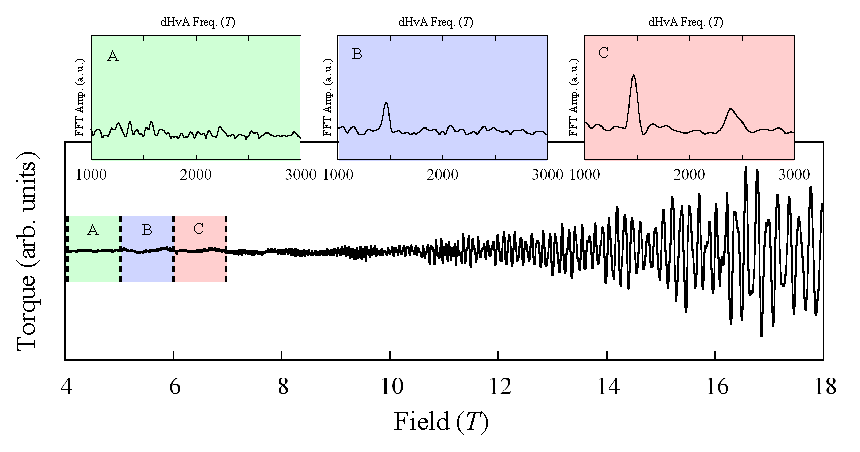
\includegraphics[scale=0.7]{Chapter-dHvABaFe2P2/Figures/AngleDepMeasurements/RawOscillations/RawOscillations}
        \caption{An example of the torque data taken with field aligned at \unit{26}{\degree} on the reverse side of the $[001]$ to $[100]$ angle sweep detailed later. Insets show a \acp{FFT} of the data between \unit{4-5}{\tesla}, \unit{5-6}{\tesla} and \unit{6-7}{\tesla} respectively. These intervals are marked on the main plot as A, B and C.}
        \label{Fig:ResD:RawOscillations}
    \end{center}
\end{figure}

Figure~\ref{Fig:ResD:ComparisonSweepRates} shows some example Fourier transforms of data taken at various field sweep rates and plotted with the frequencies shifted arbitrarily for ease of comparison. The difference in amplitude between the sweeps at \unit{0.05}{\tesla\reciprocal\minute} and \unit{0.1}{\tesla\reciprocal\minute} is less than \unit{1}{\%} whereas the difference when sweeping at \unit{0.2}{\tesla\reciprocal\minute} is nearly \unit{5}{\%}. Unless otherwise stated, subsequent sweeps were performed at \unit{0.15}{\tesla\reciprocal\minute} at the edge of where the sweep rate makes a significant difference in amplitude.

\begin{figure}[htbp]
    \begin{center}
        \includegraphics[scale=0.9]{Chapter-dHvABaFe2P2/Figures/AngleDepMeasurements/SweepRateComparison/SweepRateComparison}
        \caption{\acp{FFT} showing the peak from the smaller branch of band $3$ taken at, A: \unit{0.05}{\tesla\reciprocal\minute}, B: \unit{0.1}{\tesla\reciprocal\minute} and C: \unit{0.2}{\tesla\reciprocal\minute}. The peaks are arbitrarily shifted in frequency for ease of comparison. Measurements taken with $H$ at \unit{10}{\degree} from $[001]$ in the $[110]$ direction.}
        \label{Fig:ResD:ComparisonSweepRates}
    \end{center}
\end{figure}

In order to make a reasonable determination of the Fermi surface of a material, an appropriate number of angle sweeps need to be made to adequately constrain the shape of the Fermi surface. Since \BaFeP is a tetragonal system, any sweep from the azimuthal direction $[001]$ down the polar plane effectively expands to four due to the fourfold symmetry. Measurements were taken at one degree intervals from $H\parallel[001]$ down to $H\parallel[100]$ and from $H\parallel[001]$ down to $H\parallel[110]$ which, in this system, effectively amount to eight sweeps.

\begin{figure}[htbp]
    \begin{center}
        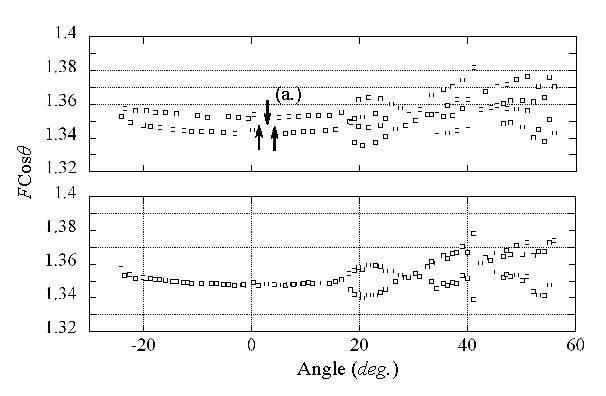
\includegraphics[scale=0.9]{Chapter-dHvABaFe2P2/Figures/AngleDepMeasurements/HysteresisCorrection/HysteresisCorrection}
        \caption{The plots show the $F\cos \theta$ for the $\alpha$ branch in the $[100]$ direction. Top panel shows the branch with the hysteresis due to field sweep direction, the bottom panel shows the data after the linear adjustment described in the main text. Arrows at point (a.) show how the points were shifted.}
        \label{Fig:ResD:HysteresisCorrection}
    \end{center}
\end{figure}

In general, runs were performed with an excitation voltage of \unit{1}{\volt}. To ensure that there was no self heating effects, runs were also performed with an excitations voltage of \unit{0.5}{\volt} and \unit{2}{\volt} at $T\approx\unit{0.6}{\kelvin}$ (where we expect the \ac{LK} curve to be steep) and no change in oscillation amplitude due to heating was observed.

The magnetic field was alternatively ramped up and then down meaning subsequent measurements were generally performed with the magnetic field ramping in opposite directions. Although in theory this should not affect the results in any way, subsequent \ac{FFT} peaks appeared to alternately be shifted by up to $\sim\pm\unit{21}{\tesla}$ with the magnitude of the shifts being roughly proportional to frequency. Assuming that the shifts were an artefact of the measurements, a linear correction determined by visual inspection was applied of $F_{\textrm{corr.}} = 3 + \frac{10}{8000} F_{\textrm{meas.}}$ for the sweep in the $[100]$ direction and $F_{\textrm{corr.}} = 0 + \frac{21}{8000}  F_{\textrm{meas.}}$ and  $F_{\textrm{corr.}} = 0 + \frac{18}{8000} F_{\textrm{meas.}}$ for the two sets of measurements performed to complete the sweep in the $[110]$ direction. Figure~\ref{Fig:ResD:HysteresisCorrection} shows an example of these hysteric shifts and the subsequent correction applied.

\begin{figure}[htbp]
    \begin{center}
        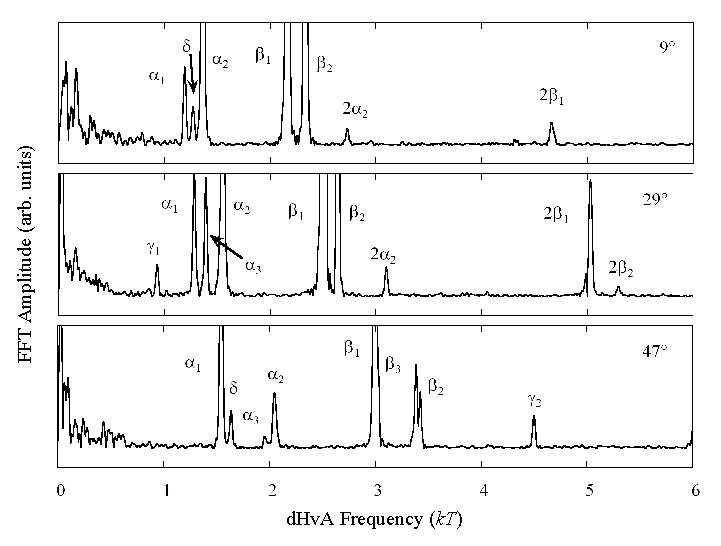
\includegraphics[scale=0.7]{Chapter-dHvABaFe2P2/Figures/AngleDepMeasurements/FFTExamples/FFTExamples}
        \caption{\ac{FFT} after a second order polynomial background was subtracted at various labelled angles between $[001]$ and $[110]$. The labels for peak identification are explained in the next section.}
        \label{Fig:ResD:FFTExamples}
    \end{center}
\end{figure}

Figure~\ref{Fig:ResD:FFTExamples} shows three example \acp{FFT} which show peaks from all the principal bands identified the next section. They also show first and second harmonics\footnote{Third harmonics were also identified in other \acp{FFT}, these are shown in figure~\ref{Fig:ResD:AngleSweepMeasured}.}. The low frequency region in figure~\ref{Fig:ResD:FFTExamples} shows noise from the cantilever, but according to \ac{DFT} fits performed in the next section, this region also likely contains signal from the minimum of band $1$. Given that the signal from electron bands is generally small due to high scattering rate, we were not able to extract a convincing Fourier peak.

Figure~\ref{Fig:ResD:AngleSweepMeasured} shows the \ac{FFT} frequency of peak data multiplied by $\cos\theta$ after having the angle determined as described in section~\ref{Sec:Exp:AngleCorrection}.  Signal can be observed up to relatively high angles with peak observed almost up to $80\degree$ in the $[110]$ direction which, along with the observation of third harmonics, and the onset of oscillations in relatively low field is testament to the high quality of the crystal.

\begin{figure}[htbp]
    \begin{center}
        \includegraphics[scale=0.9]{Chapter-dHvABaFe2P2/Figures/AngleDepMeasurements/AngleSweepMeasured/AngleSweepMeasured}
        \caption{Peaks identified by varying the field range, window type and background polynomial. Left panel shows data taken with the field parallel to $[001]$ down to $[110]$, the right panels shows $[001]$ to $[100]$.}
        \label{Fig:ResD:AngleSweepMeasured}
    \end{center}
\end{figure}

The left panel in figure~\ref{Fig:ResD:IdentifyingBands} shows the measured rotation data (circles) for the plots towards the $[100]$ direction and in addition the data from the $x=0.63$ data in the \BaFePAs series multiplied by amounts commensurate to the expected shifts in the Shishido paper~\cite{Shishido2010} (black squares). We can see that while the size of the areas changes between the two values, the overall shape of the $x=0.63$ data matches reasonably well with the data for $x=1$ for bands 2, 3 and 4 at least. Assuming that nothing exotic happens in the intermediary, we can extrapolate the shape of these Fermi surfaces across the range by applying the known electron Fermi surface areas and the compensation condition. This is explored further in the next section.

\begin{figure}[htbp]
    \begin{center}
        \includegraphics[scale=1.0]{Chapter-dHvABaFe2P2/Figures/AngleDepMeasurements/IdentifyingBands/IdentifyingBands}
        \caption{Left panel shows the measured data with points overlaid from BaFe$_2$(As$_{0.37}$P$_{0.63}$)$_2$~\cite{Analytis2010c} with the $\alpha$ and $\gamma$ frequencies multiplied by $1.33$ and $\beta$ frequencies multiplied by $1.19$ commensurate with known shifts from literature. Right panel shows \ac{DFT} calculations (lines) overlaid on top of measured \ac{FFT} data (circles). Data is colour coded according to the corresponding bands. Points in grey are harmonics.}
        \label{Fig:ResD:IdentifyingBands}
    \end{center}
\end{figure}



\subsubsection{Rigidly shifting the calculated \ac{DFT} energies}
    \label{Sec:ResD:DFTShifts}

The right panel of figure~\ref{Fig:ResD:IdentifyingBands} shows the \ac{DFT} calculations performed using the augmented plane wave method plus local orbits method method as implemented in the WIEN2k package~\cite{Blaha2001}. The unit cell used was that measured by Mewis et al. which are listed in table~\ref{Table:ResD:LatticeParams} and the subsequent \ac{DFT} calculations were processed into rotation plots using Ed's MATLAB code. Results are shown superimposed over the measured data. By factoring the frequency with $\cos{\theta}$ it becomes clearer which of the orbits is a maximal extrema and which is a minimal extrema. Using this knowledge as well as clues from the Fourier amplitude of the measured data, it was possible to separate out individual bands which have been colour coded and labelled --- according to literature convention --- as specified in table~\ref{Tab:ResD:BandNaming}. Minimal extrema are sub-labelled $1$, maxima are sub-labelled $2$. The points marked in grey are the harmonics which were identified by overlaying the measured data on itself after doubling and tripling of the frequency.

\begin{table}
    \begin{center}
        \caption{A summary of the Fermi surface labelling used.}
        \begin{tabular}[htbp]{llll}
\toprule
Band Num.  & Label & Colour    & Type \\
\midrule
1   & $\delta$  & Orange    & hole \\
2   & $\gamma$  & Red   & hole \\
3   & $\beta$   & Blue  & electron \\
4   & $\alpha$  & Green & electron \\
\bottomrule
        \label{Tab:ResD:BandNaming}
        \end{tabular}
    \end{center}
\end{table}

As with previous \ac{DFT} calculations in the \BaFePAs series, the calculated values are consistently higher than the measured values~\cite{Shishido2010}. The exception in this case is $\gamma_2$ which is not much different from the calculated values.

As is shown in the right panel of figure~\ref{Fig:ResD:IdentifyingBands}, the rotation plots from the \ac{DFT} calculations match up qualitatively with the data but do not match up quantitatively -- the electron bands overestimating the size of the measured extremal orbits. 

\begin{figure}[htbp]
    \begin{center}
        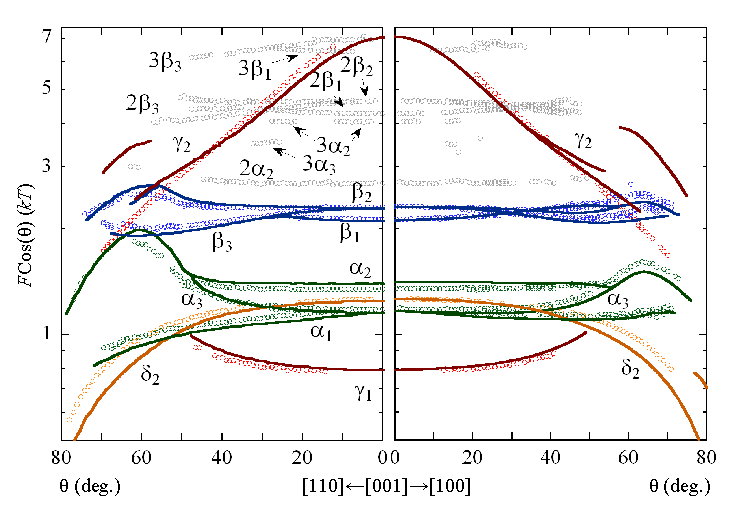
\includegraphics[scale=0.9]{Chapter-dHvABaFe2P2/Figures/AngleDepMeasurements/AngleSweepRigidShift/AngleSweepRigidShift}
        \caption{\ac{dHvA} frequencies multiplied by $\cos(\theta)$. Solid lines are rigidly shifted \ac{DFT} calculations, open circles are measured data. $H$ field directed along $[001]$ towards (a.) $[001]\rightarrow[100]$ and (b.) $[001]\rightarrow[110]$.}
        \label{Fig:ResD:AngleSweepRigidShift}
    \end{center}
\end{figure}

In order to obtain the correct shape of Fermi surface, the \ac{DFT} calculations need to be tweaked. One technique is to apply small band-specific rigid energy shifts, which, in most cases is enough to bring the \ac{DFT} in line with the experimental data. Figure~\ref{Fig:ResD:AngleSweepRigidShift} shows the rotation plots which rotate towards both the 100 and 110 directions along with appropriately shifted calculations. Table~\ref{Tab:ResD:EnergyShifts} lists those energy shifts.
\begin{table}
    \begin{center}
        \caption{Rigid energy shifts required to match the \ac{DFT} calculations with the measured data.}
        \begin{tabular}[htbp]{llr}
\toprule
Band    & \multicolumn{2}{l}{Energy Shift (Ry)} \\
\midrule
1       &       & -0.0083      \\
2       & Wide  & 0.0          \\
        & Narrow & -0.0038     \\
3       &       & 0.0043       \\
4       &       & 0.0050        \\
\bottomrule
        \label{Tab:ResD:EnergyShifts}
        \end{tabular}
    \end{center}
\end{table}

Band $2$ in this case has two separate shifts specified in two different regions of the \ac{BZ}. The rotation plot for the wider orbit located at the edge of the \ac{BZ} was calculated with no energy shift and the narrow part of the Fermi surface around the $\Gamma$ point was calculated with a shift of $\unit{0.0038}{\textrm{Ry}}$. This provides a reasonable match for the rotation plot where we can apply the shift to the two regions discretely, however is proves problematic when we wish to study intermediate areas since it is not clear how the Fermi surface varies between the two regions. A technique for applying appropriate energy shifts throughout the \ac{BZ} is explored in the next section.

\begin{figure}[htbp]
    \begin{center}
        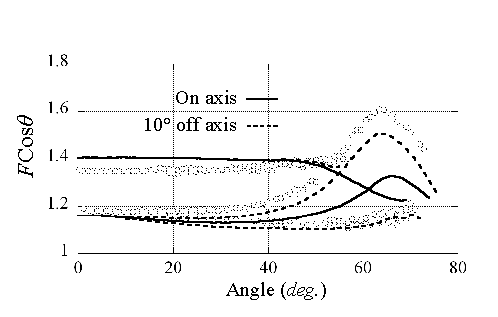
\includegraphics[scale=0.9]{Chapter-dHvABaFe2P2/Figures/AngleDepMeasurements/BaselMisalignment/BaselMisalignment}
        \caption{Portion of the measured \ac{FFT} peaks taken towards the `$[100]$' direction. Superimposed is angle plots calculated from \ac{DFT}. Solid is calculated for the field rotating down to $[100]$, dotted is rotated down to \unit{10}{\degree} off $[100]$ in the basel plane.}
        \label{Fig:ResD:BaselMisalignment}
    \end{center}
\end{figure}
For the $[100]$ direction it became apparent from the fact that the \ac{DFT} and the measured curves were qualitatively different that the field was not perfectly aligned with the $[100]$ axis of the sample. Figure~\ref{Fig:ResD:BaselMisalignment} shows how the measured data (circles) does not align well with the plots calculated for rotations towards $[100]$ (solid) but does align well with plots towards an axis which is rotated \unit{10}{\degree} within the $ab$-plane from the $[100]$ direction. A \unit{10}{\degree} misalignment is within the estimated basel alignment error for the microscope images. The data will continue to be labelled as in the $[100]$ plane however for convenience.

In the first place, these shifts were applied as they conveniently and effectively corrected the Fermi surface energies, however the question arises as to whether there is any physical significance to be attached to them. The technique of rigid energy corrections has been applied to previous measurements on LaFePO~\cite{Carrington2009} and SrFe$_2$P$_2$~\cite{Analytis2009} both of which are highly two dimensional systems that exhibit relatively strong nesting characteristics. This is in contrast with measurements on CaFe$_2$P$_2$~\cite{Coldea2009} which has a highly three dimensional Fermi surface and no nesting vector. Furthermore the bulbous area of the three dimensional hole surface in \BaFeP which does not nest requires no shifting of the Fermi surface to match \ac{DFT} calculations, whereas the nested neck portion does require a shift. This correlation between nesting and shifts in calculated energy make the spin-density-wave fluctuations that are associated with the nesting phenomena an obvious candidate for the cause of the discrepancy between \ac{DFT} calculation and experiment.


\subsubsection{Shifting the \ac{DFT} calculations proportional to orbital character}
\label{Sec:ResD:ShiftingDFTPropToOrbitalCharacter}

Figure~\ref{Fig:ResD:Band2DCharacterVsKz} shows the partial orbital character for for each of the bands along the path of Fermi surface contour in a $[110]$ slice through the \BaFeP \ac{BZ} as a function of $k_z$. The top row of plots show the character broke down by atomic contribution, the middle row is broken down by the $s$, $p$, $d$ and $f$ contributions to the iron contribution and the bottom row breaks down the iron $d$ character into its sub orbitals.
\begin{figure}[htbp]
    \begin{center}
        \includegraphics[scale=0.95]{Chapter-dHvABaFe2P2/Figures/AngleDepMeasurements/BandCharacterVsKz/AllBandCharacterVsKz}
        \caption{Partial orbital characters along the Fermi surface contour in the 110 slice (shown in insets) vs. $k_z$. Top row is the character broken down by each atom, middle row is the iron contribution broken down into the $l$ orbital contributions, the bottom row is the iron $d$ orbital contributions broken down into its suborbitals. The leftover region in the top row is made up of the interstitial regions outside of the muffin tin spheres which are not associated with any particular atom.}
        \label{Fig:ResD:Band2DCharacterVsKz}
    \end{center}
\end{figure}

The interstitial regions account for about \unit{20--32}{\%} of the electron band character along suggesting that they may have higher mobility than the hole bands. Which would explain why the oscillations from the electron bands are much stronger in the \ac{dHvA}. The hole bands range between \unit{8--18}{\%} with band 1 being more mobile around the $\Gamma$ point whilst band 2 being higher around the $Z$ point at the top edge of the \ac{BZ}.

We can see the vast majority of Fermi surface character is due to the iron atomic contributions with some phosphor for bands 2 and 3 which corresponds well to the notion of FeP conducting planes. For all the bands, the overwhelming majority of the contribution from the iron atoms is from the $d$ orbitals and so other contributions are ignored.

Band $2$ has very little basel-plane \Dxy and \DxTwoyTwo character close to the Fermi level but shows a significant amount of \DzTwo character at the wide region of the Fermi surface and \DxzDyz character at the narrow region. Evidently, energy shifts could be applied which are scaled to either the \DzTwo and \DxzDyz orbital character in order that we obtain a smooth energy shift transition between the narrow and wide regions discussed previously. 

Energy shifts were applied across the full three dimensional \ac{BZ} for band $2$ using the following two scalings which were determined by trial and error fitting of the data,
%%
\begin{align*}
\textrm{\DzTwo:}\quad \Delta\epsilon &= 0.002 - 0.0052 \left[1 - \frac{\epsilon - 0.033}{0.2205 - 0.033}\right] \\
\textrm{\DxzDyz:}\quad \Delta\epsilon &= 0.002 - 0.0052 \left[\frac{\epsilon - 0.0946}{0.3135 - 0.0946}\right]
\end{align*}
%%
Note that these scalings ensure that the energy shift applied varies between \unit{-32}{\milli\textrm{Ry}} and \unit{2}{\milli\textrm{Ry}} which are slightly different to the values applied when rigidly shifting the band. This is due to the fact that the Fermi surface area measured in the narrow region is affected more and more by the size of the Fermi surface in the wide region (and vice-versa) as the azimuthal angle gets higher. The calculated area deviates from the measured area which results in the crossing of the calculated rotation plot with the measured rotation plot shown in the first panel of figure~\ref{Fig:ResD:Band2DCharacterRigidComparison}. So when the rigid shifts were being determined, values were chosen which best lines up along the full length of the curve -- one which will be slightly lower than if we were to match the plots exactly at $\theta=0^\circ$.

\begin{figure}[htbp]
    \begin{center}
        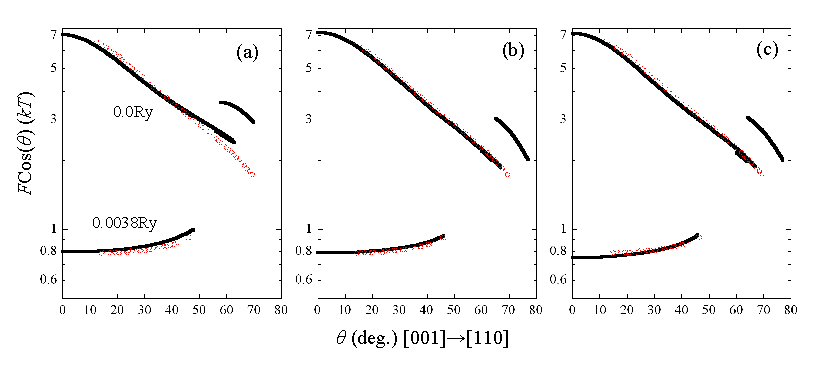
\includegraphics[scale=0.8]{Chapter-dHvABaFe2P2/Figures/AngleDepMeasurements/BandCharacterRotPlot/Band2_110_RotPlot_Comparison}
        \caption{dHvA frequencies for band 2 multiplied by the cosine of the angle of the $H$ field. $H$ field directed along $[001]\rightarrow[110]$. Open circles are measured data, solid lines represent (a) rigidly shifted \ac{DFT} calculations, (b) \ac{DFT} calculations shifted proportional to \DzTwo orbital character, (c) \ac{DFT} calculations shifted proportional to \DxzDyz orbital character.}
        \label{Fig:ResD:Band2DCharacterRigidComparison}
    \end{center}
\end{figure}

The second and third panels of figure~\ref{Fig:ResD:Band2DCharacterRigidComparison} show the rotation plots calculated with the energy shifts applied proportional to \DzTwo and \DxzDyz orbital character respectively. We observe a much better alignment of the measured and calculated data for all angles. Figure~\ref{Fig:ResD:BandCharacterFSShiftComparison} shows the Fermi surfaces before and after shifting using the rigid energy shifts for bands $1$, $3$ and $4$ and using shifts scaled to \DzTwo orbital character for band $2$. Figure~\ref{Fig:ResD:FullBandCharacterFermiSurface} shows the assembled unit cell for \BaFeP from the corrected \ac{DFT} calculations and figure~\ref{Fig:ResD:ShiftedBandStructure} shows the shifted band structure for the bands that cross the Fermi level.
%%
\begin{figure}[htbp]
    \begin{center}
        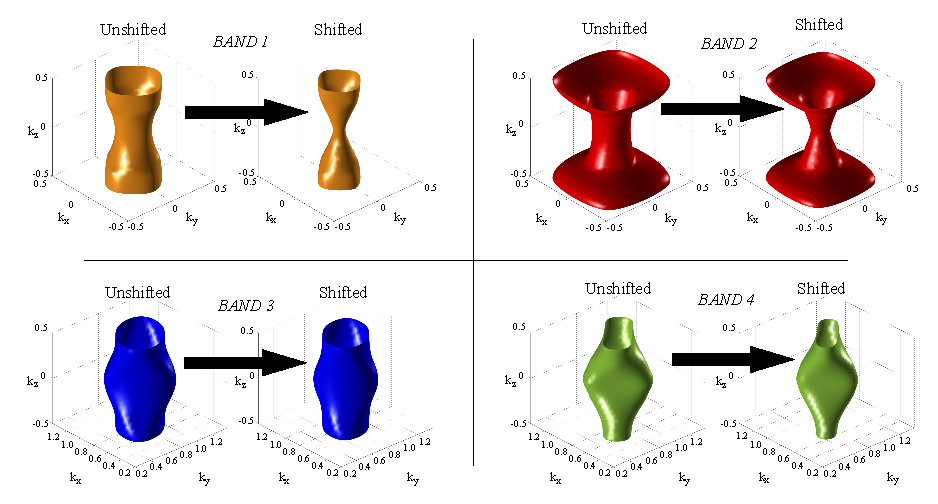
\includegraphics[scale=0.8]{Chapter-dHvABaFe2P2/Figures/AngleDepMeasurements/BandCharacterFermiSurface/BandCharacterFermiSurfaceShiftComparison}
        \caption{Comparison of Fermi surfaces according to \ac{DFT} calculations both before and after shift corrections are applied. Rigid shifts are applied to bands 1, 3, 4 and shifts proportional to \DzTwo character are applied to band 2.}
        \label{Fig:ResD:BandCharacterFSShiftComparison}
    \end{center}
\end{figure}
%%
\begin{figure}[htbp]
    \begin{center}
        \includegraphics[scale=0.7]{Chapter-dHvABaFe2P2/Figures/AngleDepMeasurements/BandCharacterFermiSurface/FullBandCharacterFermiSurface}
        \caption{Fully assembled Fermi surface in the first \ac{BZ} of \BaFeP as determined by \ac{DFT} calculations corrected by either rigid energy shifts (bands 1, 3, 4) or shifts proportional to \DzTwo character (band 2)}
        \label{Fig:ResD:FullBandCharacterFermiSurface}
    \end{center}
\end{figure}
%%

The final corrections show the \ac{DFT} calculations being adjusted in size only for the electron and inner hole surfaces with overall shrinking of volume, the outer hole surface is adjusted in shape as well. Volume calculations as a percentage of the \ac{BZ} are given for each of the Fermi surfaces before and after shifting in table~\ref{Table:ResD:FermiSurfaceVolumes},
\begin{table}
    \begin{center}
           \caption{Volumes of the shifted and unshifted Fermi surfaces as a percentage of \ac{BZ} volume.}
        \begin{tabular}[htbp]{lrrr}
\toprule
Band    & Unshifted    & Shifted \DzTwo    & Shifted \DxzDyz \\
\midrule
1  & 5.54\%    & 2.28\%    & 2.28\%    \\
2  & 10.37\%   & 9.74\%    & 9.64\%    \\
3  & (-)9.58\% & (-)7.89\% & (-)7.89\% \\
4  & (-)6.39\% & (-)4.49\% & (-)4.49\% \\
\midrule
Total & -0.065\%    & -0.352\%  & -0.450\%  \\
\bottomrule
        \label{Table:ResD:FermiSurfaceVolumes}
        \end{tabular}
    \end{center}
\end{table}
The volumes compensate better before the shifts by a small amount ($\sim$\unit{0.4}{\%}) with the shifts proportional to \DxzDyz being slightly closer to the unshifted volume.

\section{Obtaining the Fermi surface for members of the \BaFePAs series}

We can use existing literature measurements of the Fermi surface at $x=0.38$ from Yoshida \etal~\cite{Yoshida2010}, $x=0.63$ from Analytis \etal~\cite{Analytis2010c} and a range between $0.4 < x < 1.0$ from Shishido \etal~\cite{Shishido2010} to obtain an approximate relation for the size of Fermi surface orbits across the \BaFePAs series. Figure~\ref{Fig:ResD:SeriesRecipe} shows the maximum and minimum orbit sizes with the field along the $c$-axis from these papers along with data presented in this thesis.
\begin{figure}[htbp]
    \begin{center}
        \includegraphics[scale=1.1]{Chapter-dHvABaFe2P2/Figures/AngleDepMeasurements/SeriesRecipe/SeriesRecipe}
        \caption{Left panel shows the trend in electron orbit size at $\theta=0\degree$ over the series, right panel show the hole orbit size trends. Dotted lines show linear fits to the data.}
        \label{Fig:ResD:SeriesRecipe}
    \end{center}
\end{figure}
It may be possible to apply a linear scaling to determine the intermediate orbit sizes however there are a number of assumptions that need to be made. 

Firstly we cannot apply Vegard's law beyond a structural transition in the series meaning we cannot extrapolate to the orthorhombic state at the low $x$ end of the phase diagram. The measurement by Yoshida et al. at $x=0.38$ roughly coincides with the edge of the orthorhombic transition as shown in figure~\ref{Fig:Intro:PhaseDiagram} but was found to be tetragonal and so we can use to to define the lower limit for the extrapolation at low temperatures. There is also a so called `collapsed tetragonal phase' which occurs in the \BaFeAs at a pressure \unit{27}{\giga\pascal}~\cite{Mittal2011} at \unit{33}{\kelvin} which could present a problem as we apply chemical pressure. The optimal \Tc of \BaFeAs under pressure is $\sim$\unit{5}{\giga\pascal}~\cite{Colombier2009} and optimal \Tc for the \BaFePAs series is $x\sim0.3$, and so we can very approximately place $x=1$ corresponding to $\sim$\unit{7}{\giga\pascal} which is about half of that required for the collapsed phase transition. Moreover the author is not aware of any reports of the collapsed phase being observed in the \BaFePAs series at atmospheric pressure and so we assume that this is the case. 

There is also the problem of the third hole surface around the $\Gamma$ point which appears in \ac{DFT} calculations. Although it has not been observed in any of the measurements, this is to be expected since electron surfaces generally scatter more and so have a weaker signal to electron pockets and also it may be close in size and shape to other hole surfaces making it difficult to pick out with current \ac{ARPES} resolution.

Looking at figure~\ref{Fig:ResD:SeriesRecipe} we see some inconsistencies which may also throw some doubt onto such a linear fit. Key points from Yoshida \etal are measured from \ac{ARPES} and not \ac{dHvA}. As they were measured at \unit{10}{\kelvin}, this means that the Fermi surface is measured in the superconducting state and not the field suppressed normal state which is the case for the \ac{dHvA} data. It is not clear if this results in different Fermi surfaces. It also should be noted that a linear extrapolation of $\delta$ suggests that it will become more three dimensional as it goes below $x=0.38$, however this does not appear to be supported by the \ac{DFT} results which show it remaining quasi-two dimensional. 

With the above (many) caveats in mind, we can determine a series of linear laws which would approximately determine the orbit sizes for $0.38 < x < 1.0$ by applying fits to the data in figure~\ref{Fig:ResD:SeriesRecipe}. The results of these fits are given in table~\ref{Table:ResD:SeriesRecipeFits}.
\begin{table}
    \begin{center}
           \caption{Linear relations to determine orbit sizes. Coefficients are of the form $F=mx+c$.}
        \begin{tabular}[htbp]{lrr}
\toprule
Orbit   & $m$   & $c$   \\
\midrule
$\delta_{\textrm{max}}$ & 0.081 & 1.169 \\
$\delta_{\textrm{min}}$ & -1.766 & 1.841 \\
$\gamma_{\textrm{max}}$ & 4.339 & 3.111 \\
$\gamma_{\textrm{min}}$ & 0.698 &  0.071 \\
$\beta_{\textrm{min}}$ & 0.749 & 1.352 \\
$\beta_{\textrm{max}}$ & 0.811 & 1.489 \\
$\alpha_{\textrm{max}}$ & 0.495 & 0.646 \\
$\alpha_{\textrm{min}}$ & 0.946 & 0.404 \\
\bottomrule
        \label{Table:ResD:SeriesRecipeFits}
        \end{tabular}
    \end{center}
\end{table}

